\documentclass[border=0.1cm]{standalone}
\usepackage{tikz}


\begin{document}

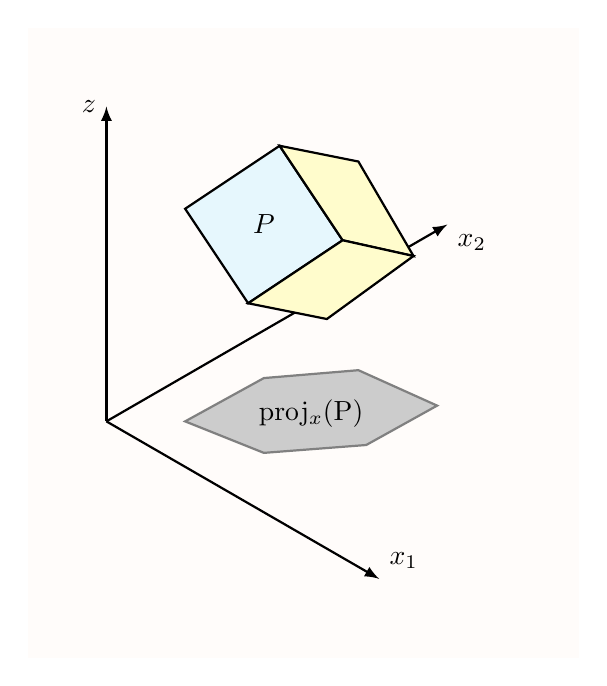
\begin{tikzpicture}
\fill[orange!2] (-1,-3) rectangle (6,5);
\draw[-latex, thick] (0,0) -- (0,4)node[left]{$z$};\draw[-latex, thick](0,0) -- (30:5)node[below right]{$x_2$};\draw[-latex, thick] (0,0) -- (-30:4)node[above right]{$x_1$};

\draw[thick,fill=cyan!10] (1,2.7) -- (2.2,3.5) -- (3,2.3) -- (1.8,1.5) -- cycle;
\draw[thick,fill=yellow!20] (2.2,3.5) -- (3.2,3.3) -- (3.9,2.1) -- (3,2.3) -- cycle;
\draw[thick,fill=yellow!20] (3.9,2.1) -- (3,2.3) -- (1.8,1.5) -- (2.8,1.3) -- cycle;
\node at (2,2.5) {$P$};

\draw[fill=black!20,thick,draw=gray] (1,0) -- (2,0.55) -- (3.2,0.65) -- (4.2,0.2) -- (3.3,-0.3) -- (2,-0.4) -- cycle;

\node at (2.6,0.1) {proj$_x$(P)};

\end{tikzpicture}

\end{document}
